\section{Analysis and Discussion}
\label{sec:analysis}
Our results show that self-improvement provides a promising path for building multimodal judges without relying on costly human annotations or stronger teacher models. In this section, we reflect on the strengths and limitations of our approach.  

\subsection{Scaling number of iterations}
\begin{figure}[h]
  \centering
  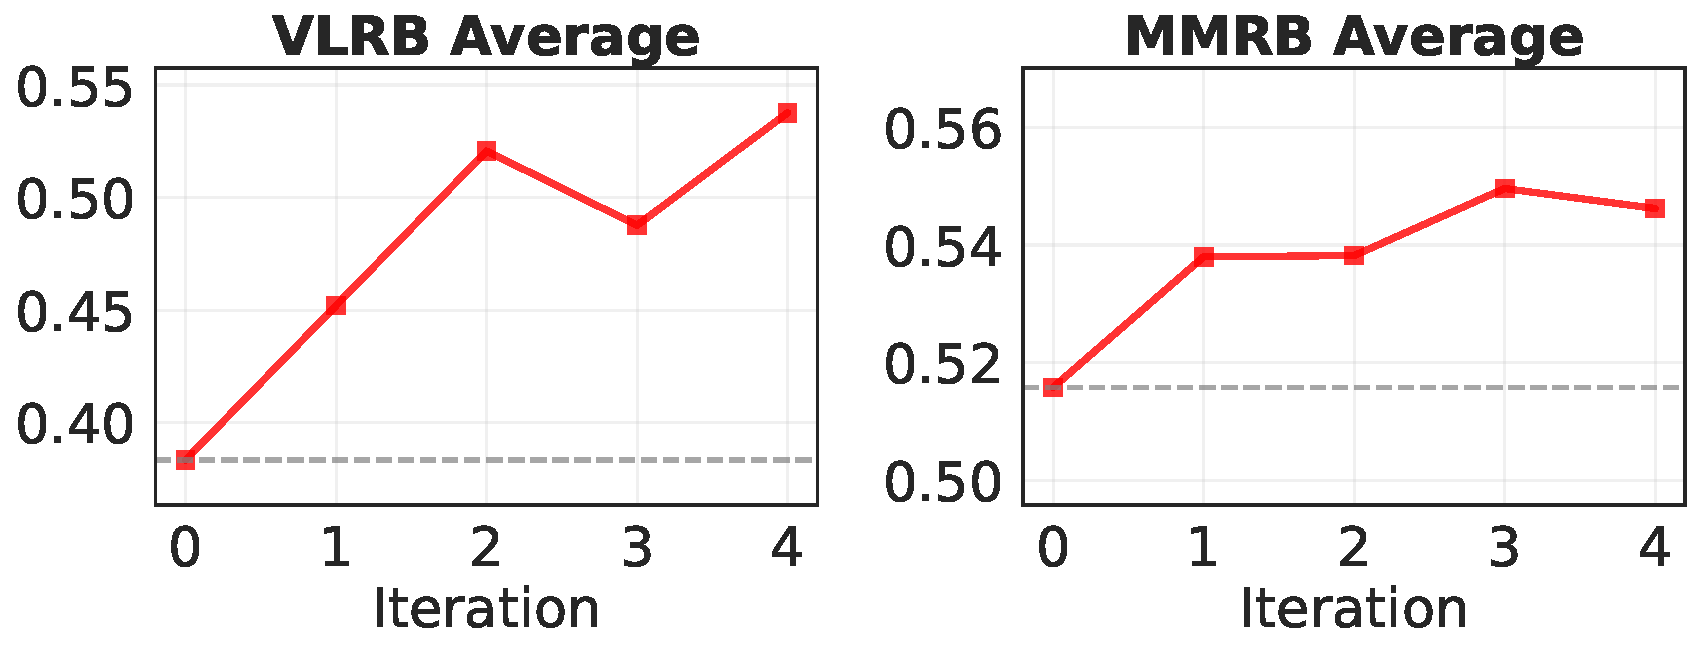
\includegraphics[width=0.70\columnwidth]{images/averaged_vlrb_mmrb_metrics_10k_data.pdf}
  \caption{Judge model performance across training iterations. The left lanel shows average VLRB scores and the right panel shows average MMRB scores. After 4 iterations, our 11B judge model is comparable with Claude-3.5 and Llama-90B on VLRB.}
  \label{fig:results_ave}
\end{figure}
 
Our iterative training scheme enables the model to \textit{generate more training data pairs at each iteration} as the judge model's performance improves. \begin{wrapfigure}{r}{0.25\textwidth}
  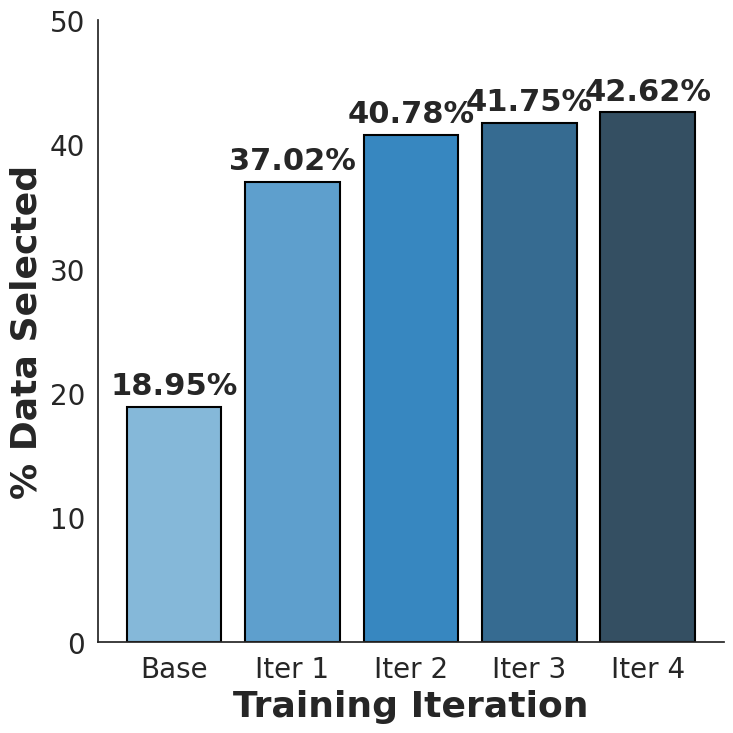
\includegraphics[width=0.25\textwidth]{images/data_perc.png}
  \caption{Increasing \% of data sampled from each training iteration}
  \label{fig:data_select_perc}
\end{wrapfigure}
Figure~\ref{fig:data_select_perc} shows that the percentage of retained training data increases from 19\% at baseline to 43\% by iteration 4, with the largest gains in early iterations. 







Beyond increasing the number of training examples, we hypothesize that \textit{the quality of reasoning also improves across iterations}. Blind manual evaluation of 20 randomly sampled examples showed later iterations 
produced superior reasoning in 55\% of cases versus 10\% for early iterations, 
confirming genuine quality improvement beyond metrics. An demonstrative example of the reasoning progression for the same pairs across training iterations are shown in Appendix~\ref{tab:reasoning_progression}.


Iterative training yields substantial improvements, with the largest gains in the first iteration (10\% average improvement across VLRB and MMRB) and continued progress in later iterations (3\% average per iteration). However, improvement rates differ across dimensions. For instance, VLRB General and Hallucination show rapid, monotonic gains, while MMRB General Correctness exhibits fluctuations. These patterns reveal that different task domains respond to iterative refinement at different rates: some capabilities converge quickly and steadily with each training cycle, while others exhibit slower or more volatile learning dynamics.





\subsection{Analysis on reasoning / VQA: filtering with majority votes v.s.correct answers}
\label{sec:analysis_reasoning}

\begin{figure}[h]
  \centering
  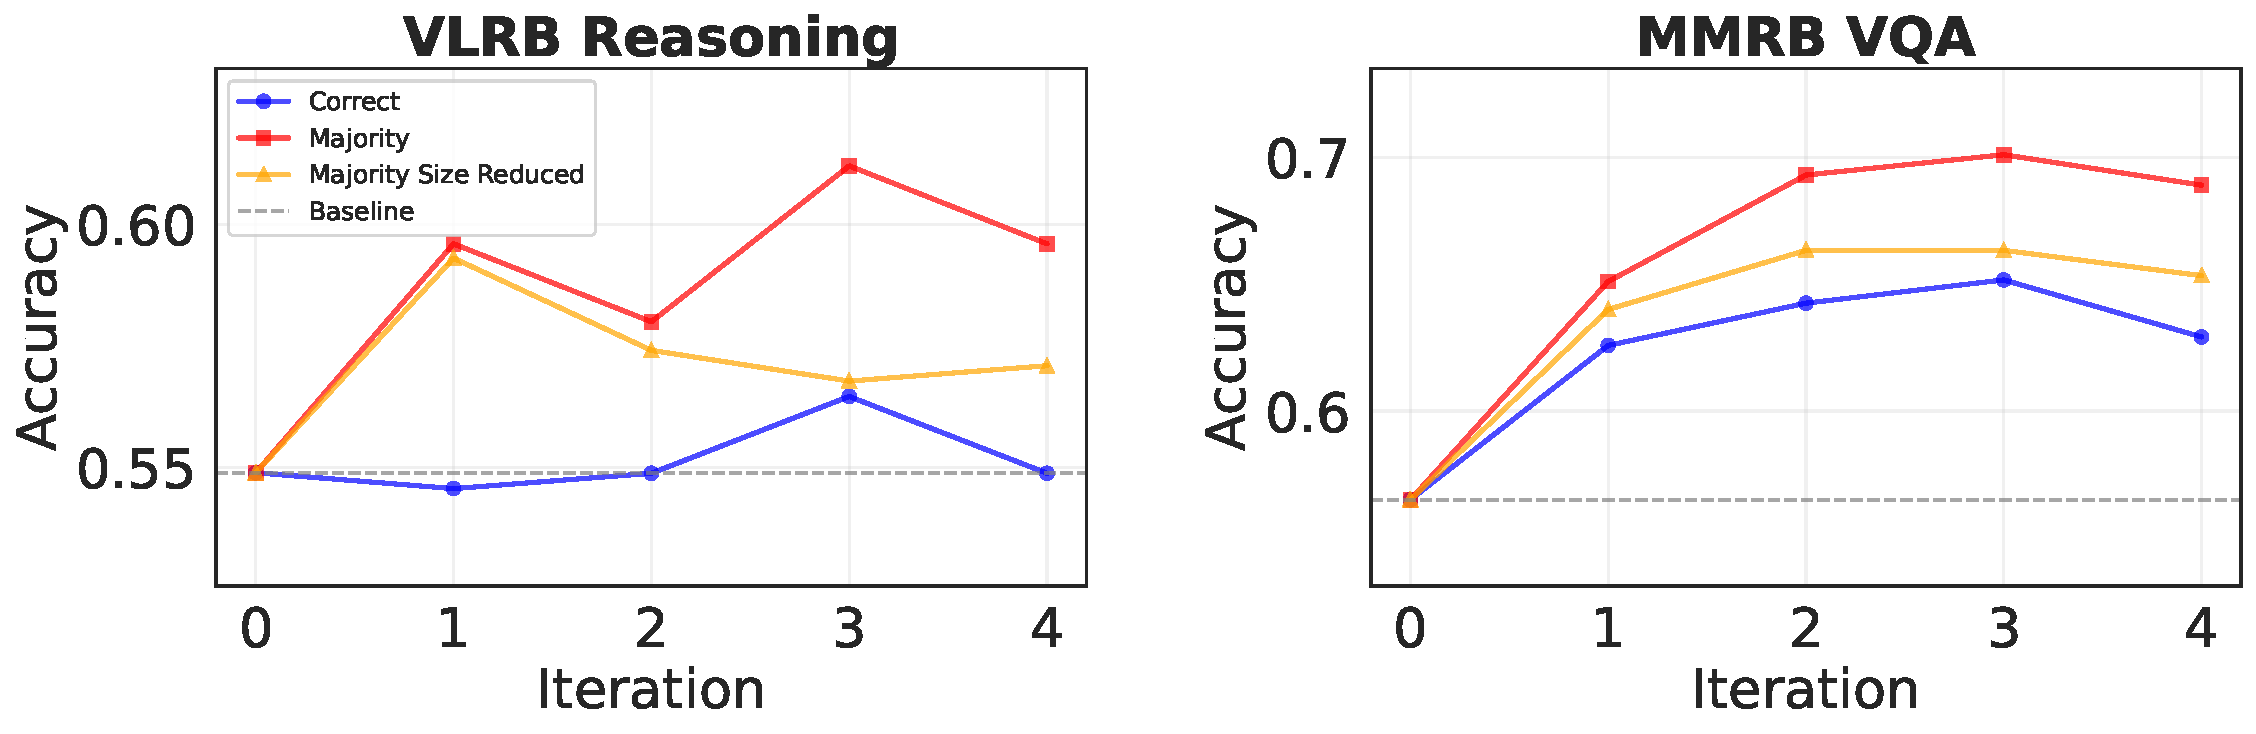
\includegraphics[width=0.70\columnwidth]{images/majority_fig.pdf}
  \caption{Performance comparing using majority voting and correct answer to filter synthetic pairs before sampling. For VLRB reasoning and MMRB VQA using majority voting to filter the synthetic pairs yields better performance after a few iterations. When reducing data size to the same with correct answer filtering, majority performance also reduced.}
  \label{fig:majority_comparison}
\end{figure}

In our preference pair synthesis, for reasoning / VQA tasks that have a short answer, we sample 16 times, and pick the majority answer as the ``preferred'' answer, and randomly sample an answer that is different as the ``less preferred'' answer. 

For ablation analysis, we also experiment with using the oracle correct answers (coming from datasets) to select the ``preferred'' answer and the ``less preferred'' answer.
Note that in the majority-voting setup, the majority answer may not be correct, especially in areas when the model struggles. 

In figure~\ref{fig:majority_comparison}, we show the comparison on dimensions where closed-ended type questions are more relevant (i.e. multiple choices, numerical answers, short answers, not captions or long answers).  On VLRB-Reasoning and MMRB-VQA, synthetic pairs constructed via majority voting yield 8.6\% and 9.5\% average improvement over correctness-filtered pairs. 


While this result may appear counterintuitive, the following underlying mechanism explains our observations. First, we find that the judge model consistently samples a greater number of data points per iteration when using majority voting compared to correctness-filtered approaches.%, as shown in \ref{fig:no_samples}. 
This increased sampling capacity provides a richer training signal during each optimization cycle. As Figure \ref{fig:majority_comparison} shows, constraining the data size of the majority set to match the correct set in each iteration reduces the performance of the original majority set. However, there still exists a gap between the performance trained with the majority set and with the correct set, which leads to our second analysis. We hypothesize that even when the judge model selects the pair containing the correct answer, this may not necessarily ensure that the judge's reasoning process is sound. For instance, in the example shown in Appendix~\ref{tab:counter_example}, the judge's reasoning prioritizes stylistic factors over factual accuracy, failing to identify that Response A contains a transcription error. Such patterns suggest that the correctness of the preferred answer does not guarantee the validity of the judgment reasoning.


While using ground truth as a filtering strategy improves judge performance in this setup, majority voting filters samples more efficiently and achieves even greater performance gains. Importantly, majority voting eliminates the dependency on ground truth labels, enabling the approach to scale to any image dataset by generating questions without requiring pre-existing answers.


\subsection{Analysis on other task dimensions}
In \S\ref{sec:analysis_reasoning}, we shows the effectiveness of our method on reasoning and VQA tasks. In this section, we analyze the performance on other task dimensions. Specifically, we focus on the categories that exhibit the most and the least significant improvements.
\label{sec:analysis_bytask}
\begin{figure}[h]
  \centering
  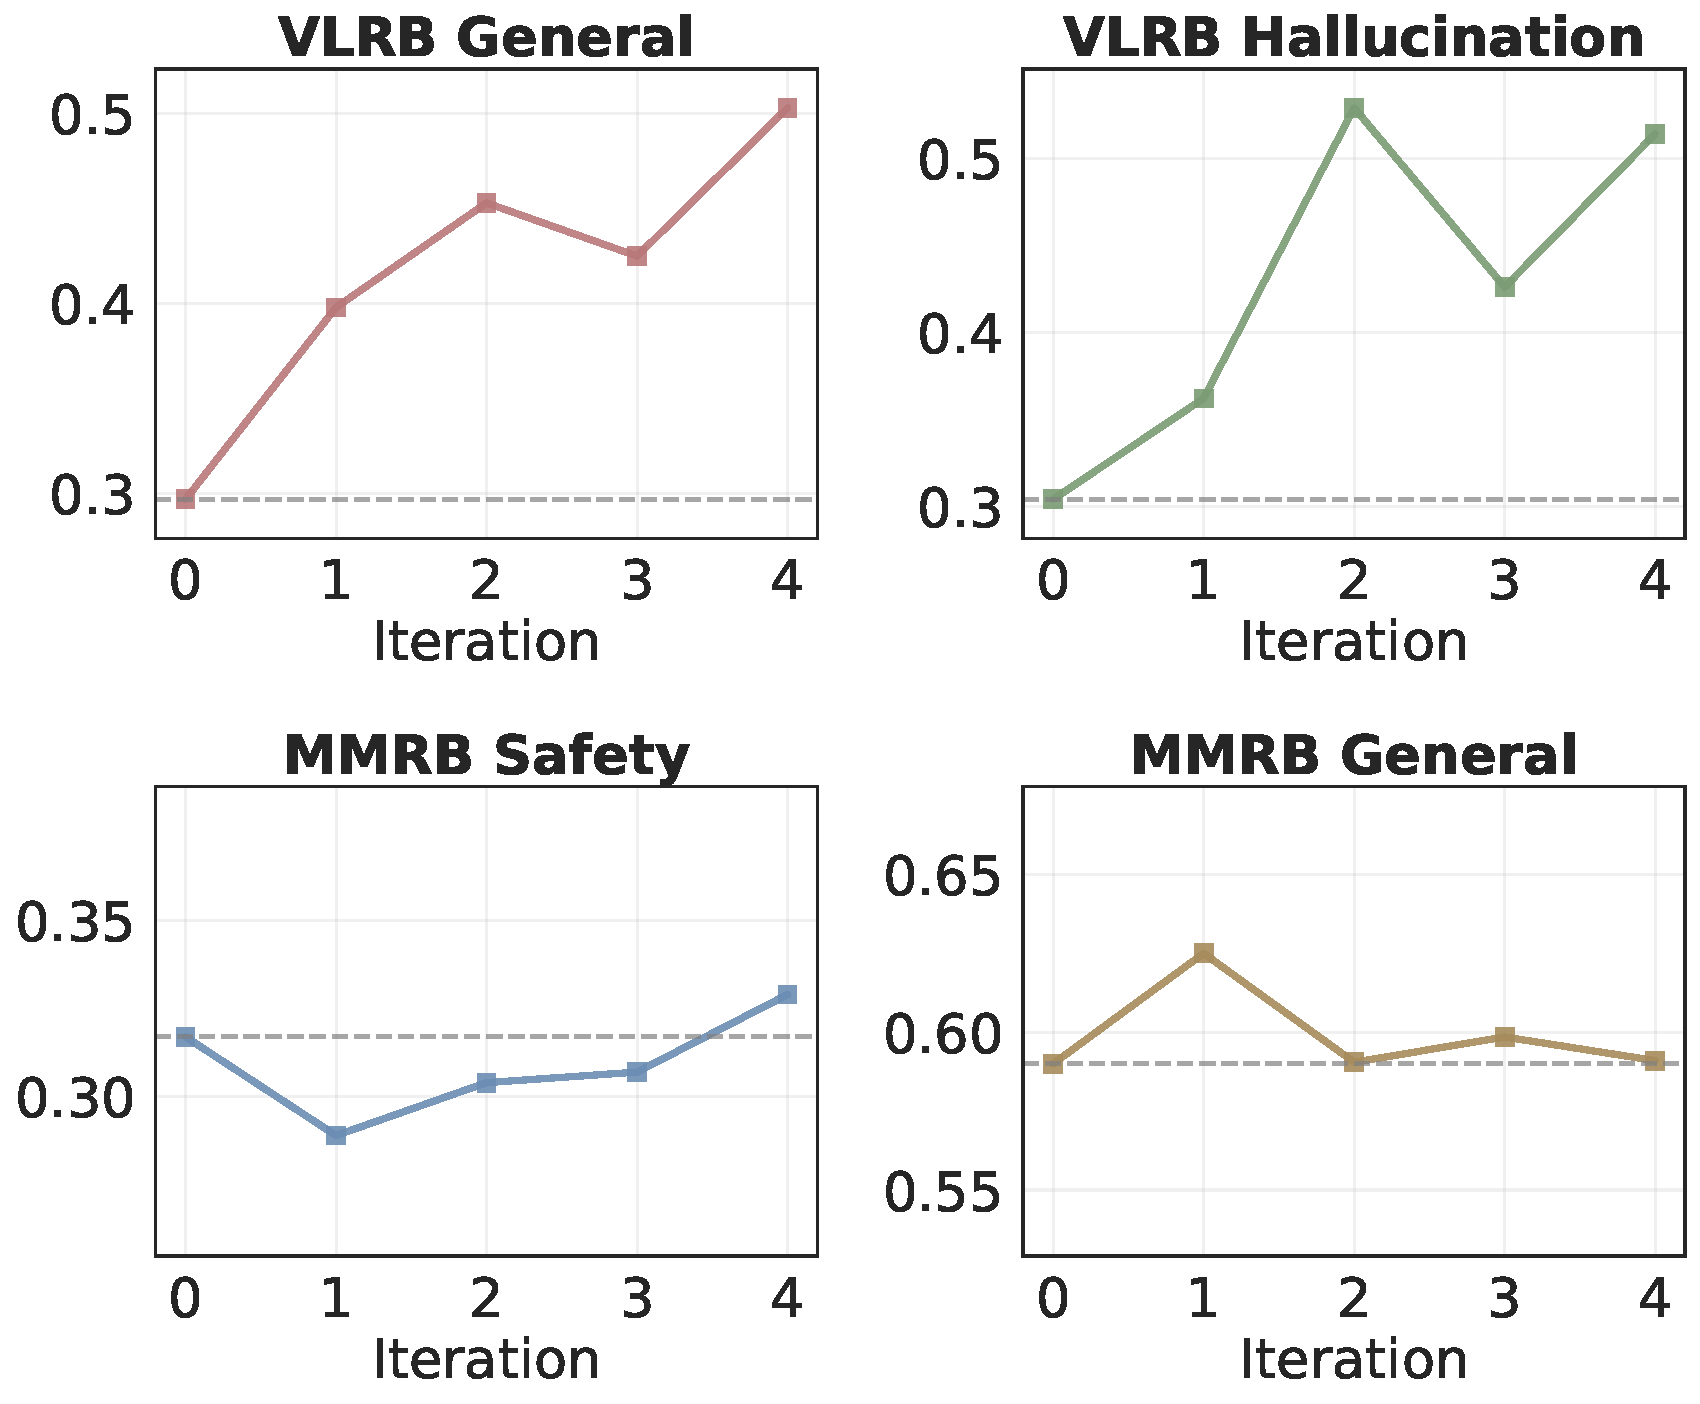
\includegraphics[width=0.60\columnwidth]{images/specific_metrics_10k_data.pdf}
  \caption{The dimensions that showed the most significant improvements (VLRB General, Hallucination) and the least significant improvements (MMRB Safety, General). More details in \S\ref{sec:analysis_bytask}.}
  \label{fig:your_label}
\end{figure}

\xhdr{VLRB General \& Hallucination} Our self-improving pipeline demonstrates particularly strong performance on VLRB general and hallucination categories. On VLRB general dimensions, our iteratively trained Llama-3.2-11B-based judge model outperforms both Llama-3.2-90B and Claude-3.5-Sonnet, while also achieving significant improvements on the hallucination dimension. These results are notable given that VLRB general draws from WildVision~\cite{lu2024wildvision} and VLFeedback~\cite{li2024vlfeedback}, which are datasets that capture authentic human preferences and diverse instruction-following scenarios from real-world VLM interactions. 
% WildVision contains genuine use cases collected from user submissions, while VLFeedback provides large-scale multi-modal instructions with comprehensive rationales. 
Our model's strong performance on this category indicates that our synthetic data generation pipeline effectively captures learning signals reflected by these real-world datasets.


\xhdr{MMRB General} The performance on MMRB General remains relatively flat compared to improvements observed in other dimensions. We hypothesize that this stems from the image diversity present in MMRB's benchmark composition. The general categories draw from two distinct datasets: NoCaps~\cite{agrawal2019nocaps} and VisitBench~\cite{bitton2023visit}. After 4 training iterations, we observe consistent performance gains on VisitBench (correctness 0.54 $\rightarrow$ 0.64), whereas NoCaps performance has either declined or plateaued (correctness 0.58 $\rightarrow$ 0.52). This divergence suggests a potential domain mismatch: NoCaps sources images from OpenImages~\cite{kuznetsova2020open}, which exhibits greater visual and object diversity for captioning tasks. The broader distribution of visual concepts in OpenImages likely challenges our model's ability to generalize beyond the training distribution. This finding underscores that both task diversity and image diversity are critical factors in synthetic data generation. While our approach successfully expands task diversity through the LLaVA-OneVision dataset~\cite{li2024llavaonevisioneasyvisualtask}, the results indicate that incorporating more diverse image sources could further enhance model robustness and generalization to visual domains such as those present in NoCaps.


\xhdr{MMRB Safety} The improvement on safety benchmarks is not as consistent as observed in other evaluation metrics. This limitation likely stems from the fact that our training data generation process did not explicitly prompt the model to produce biased or toxic content for creating synthetic pairs. The inconsistent safety performance emphasizes the critical importance of task alignment in synthetic data generation—safety improvements require training data that specifically addresses potential risks and harmful outputs. Since safety evaluation typically demands specialized guardrails and red-teaming approaches that extend beyond the scope of our current methodology, we leave comprehensive safety-focused synthetic data generation as an important direction for future work.

